\documentclass[../notes.tex]{subfiles}

\pagestyle{main}
\renewcommand{\chaptermark}[1]{\markboth{\chaptername\ \thechapter\ (#1)}{}}

\begin{document}




\chapter{The Molecular Level}
\section{Chemical Biology Introduction and the Central Dogma}
\begin{itemize}
    \item \marginnote{9/27:}Questions:
    \begin{itemize}
        \item What edition(s) of the textbook(s) should we have?
        \begin{itemize}
            \item Doesn't matter.
        \end{itemize}
        \item Will there be TA office hours?
        \begin{itemize}
            \item No.
        \end{itemize}
    \end{itemize}
    \item CHEM 233 used to be Intermediate Organic Chemistry, and CHEM 332 was the grad class. They have been merged this year because of the overlap in content.
    \item Krishnan weeks 5-7; Tang otherwise.
    \item We will not be going through reactions. The format is slides; don't try to copy them down, just make some notes. Copy them down ahead of time?
    \item Goes over the syllabus.
    \begin{itemize}
        \item No fixed textbook. Lehninger is recommended though. Whatever edition you can find.
        \item No office hours (ask questions in class or ask her to meet outside).
        \begin{itemize}
            \item Tang will show up early and stay late.
        \end{itemize}
        \item Midterms are 1 hour; final is 2 hours.
        \item Three problem sets.
        \item One in-class quiz:
        \begin{itemize}
            \item Krishnan will give us cutting-edge literature to read one week before the quiz and 5 questions.
            \item We can form study groups to discuss the questions.
            \item Multiple choice quiz on that day.
        \end{itemize}
        \item We're not supposed to memorize things in this course; the problems won't be like that.
        \item Tang may lower the exam difficulty levels from previous years.
        \item Tang doesn't want us to have to fight for points; is trying to give us a big curve so that we can just focus on learning.
        \item Since this is now only a twice a week class, Tang is cutting material on carbohydrates and protein design. May try to squeeze in orthogonal chemistry, though.
    \end{itemize}
    \item The central dogma in biology.
    \emph{picture}
    \begin{itemize}
        \item DNA $\to$ RNA $\to$ protein $\to$ needed chemical transformations.
    \end{itemize}
    \item Size in biology.
    \begin{itemize}
        \item An activity matching biological entities (e.g., E. coli, cells, RNA) to their sizes in microns.
        \item Uses the world zoom website.
        \item We may be tested on sizes, but only relative not exact (e.g., E. coli vs. a ribosome).
    \end{itemize}
    \item Red blood cells are smaller than normal cells because they don't have nuclei, and they don't need meat to divide.
    \item Concentrations in biology.
    \begin{figure}[h!]
        \centering
        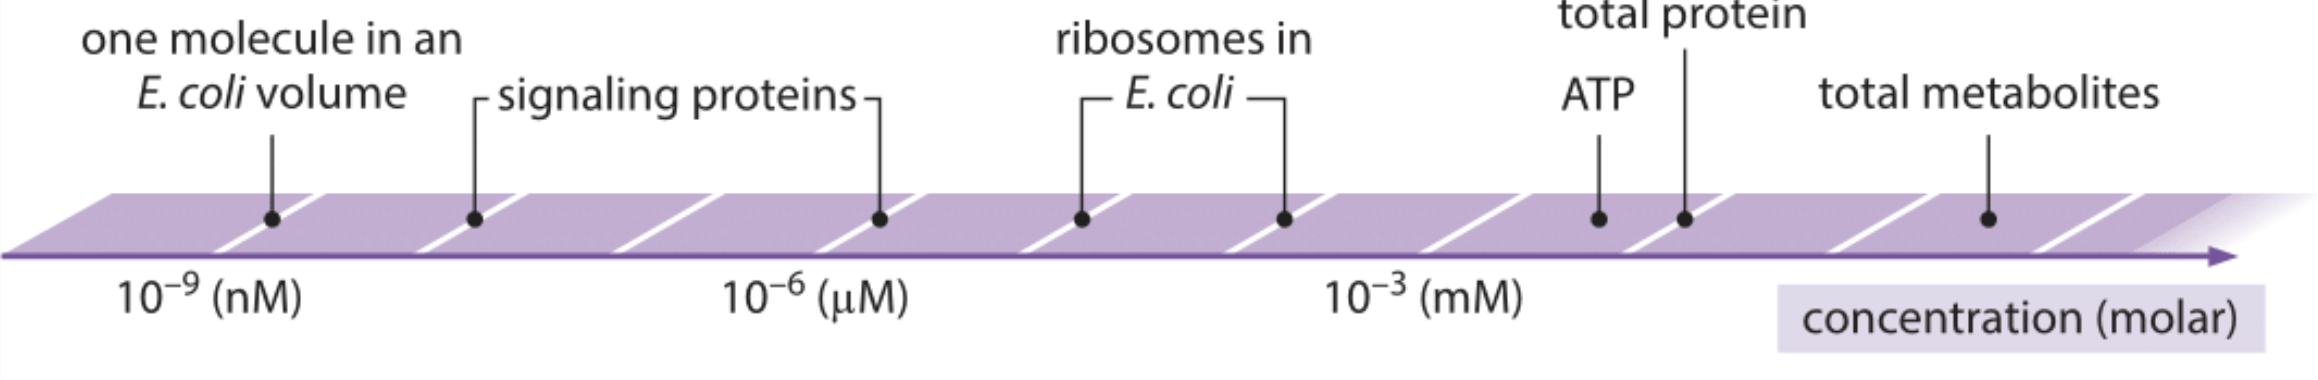
\includegraphics[width=0.9\linewidth]{../ExtFiles/bioConcentrations.png}
        \caption{Concentrations in biology.}
        \label{fig:bioConcentrations}
    \end{figure}
    \begin{itemize}
        \item You need a couple of copies of signaling proteins.
        \item Cells dedicate a lot of resources to building ribosomes.
        \item Different ions have different concentrations in different parts of the body. Additionally, different types of cells have different concentrations.
    \end{itemize}
    \item \emph{Bound} divalent ions such as \ce{Mg^2+} help cancel the charge of ATP; that's why we need them in solution.
    \item What is left after we remove all of the water from our cells?
    \begin{itemize}
        \item Largely protein, lipid, rRNA.
        \item Far more mRNA and proteins in mammalian cells than bacterial cells.
    \end{itemize}
    \item Time for protein diffusion within a cell.
    \begin{itemize}
        \item Time scale $\tau$ to traverse distance $R$ given diffusion coefficient $D$:
        \begin{equation*}
            \tau = \frac{R^2}{6D}
        \end{equation*}
        \item For a protein in cytoplasm, $D\approx\SI[per-mode=symbol]{10}{\square\micro\meter\per\second}$.
    \end{itemize}
    \item The molecular hierarchy of structure.
    \begin{itemize}
        \item The cell and its organelles are made of supramolecular complexes (e.g., the plasma membrane, chromatin, and the cell wall), which are made up of macromolecules (e.g., DNA, proteins, cellulose), which are made up of monomeric units (e.g., nucleotides, amino acids and sugars).
    \end{itemize}
    \item We will be expected to know how to draw the amino acids and nucleic acid bases.
    \item We will not talk much about lipids and sugars.
    \item Chirality and isomers review.
    \item Thalidomide.
    \begin{itemize}
        \item Was only distributed in Germany; the FDA is very proud of having picked up on the scientific malpractice and barred it from ever entering the US.
        \item Just selling one isomer doesn't work because it racemizes so quickly.
        \item Now used to treat cancer; you have to sign a bunch of paperwork saying that you won't get pregnant before you use it.
    \end{itemize}
\end{itemize}




\end{document}